\documentclass{article}
\usepackage[sexy, hdr, fancy]{evan}
\setlength{\droptitle}{-4em}

\lhead{Homework 8}
\rhead{Introduction to Statistics}
\lfoot{}
\cfoot{\thepage}

\newcommand{\var}{\mathrm{Var}}
\newcommand{\cov}{\mathrm{Cov}}

\begin{document}
\title{Homework 8}
\maketitle
\thispagestyle{fancy}

\begin{itemize}
	\item[4.] When measuring variability, we often think of it in relative terms. Suppose we define the \textit{relative variability} of a random variable to be the ratio of its standard deviation to its mean: \[r=\frac{\sqrt{\var(X)}}{E[X]}\] Suppose we observe $X_1, \cdots, X_n$ that are iid $N(\mu, \sigma^2)$ where $\mu$ and $\sigma$ re both unknown constants. If we denote the \textit{population} relative variability $r=\sigma/\mu,$ we want to test the hypothesis \[H_0:r=r_0\quad \text{v.s.}\quad H_a: r\neq r_0\] where $r_0$ is a specified constant. Under the null hypothesis the parameter $\mu$ is only constrained to be positive. Let $\theta$ denote the pair $(\mu, \sigma).$
		\begin{enumerate}[(a)]
			\item Write down the parameter space $\Theta$ for $\theta$ under $H_0\cup H_a$ and $\Theta_0$ for $\theta$ under $H_0.$
				\begin{soln}
					Under $H_0\cup H_a,$ the value $r$ can take on any real value, since for normal random variables, \[r=\frac{\sqrt{\var(X)}}{E[X]}=\frac{\sigma}{\mu}\] which can be anything. Thus, under $H_0\cup H_a,$ we have $\theta\in \RR^2.$ 

					Under $H_0,$ $\mu$ is positive, and \[r=\frac{\sigma}{\mu}=r_0\] so the parameter space is restricted to the line in $\RR^2$ corresponding to the line $\sigma=r_0 \mu.$
				\end{soln}

			\item What are the dimensions of the parameter spaces in a) and what is the difference in the two dimensions?
				\begin{answer*}
					The dimension of $\Theta$ is 2, and the dimension of $\Theta_0$ is 1, and their difference is 1.
				\end{answer*}

			\item Write down the likelihood function under the null hypothesis $H_0$ as a function of the unknown parameter $\mu$ and to keep it in a simple form, express it in terms of the quantities \[S_1=\sum_{i=1}^{n} X_i, \quad \quad S_2=\sum_{i=1}^{n} X_i^2\] 
				\begin{soln}
					Under $H_0,$ we have \[\sigma=r_0\mu\implies \sigma^2=r_0^2\mu^2\] so the distribution of $X_i$ is $N\left( \mu, r_0^2\mu^2 \right).$ Thus, the likelihood function is 
					\begin{align*}
						\prod_{i=1}^{n} \frac{1}{\sqrt{2\pi}(r_0\mu)}\exp\left( -\frac{(X_i-\mu)^2}{2r_0^2\mu^2} \right) &= \frac{1}{(2\pi)^{n/2} r_0^n \mu^n}\exp\left[ -\frac{1}{2r_0^2\mu^2}\left( \sum_{i=1}^{n} (X_i-\mu)^2 \right) \right] \\
						&= \frac{1}{(2\pi)^{n/2} r_0^n \mu^n}\exp\left( \frac{-S_2+2\mu S_1-n\mu^2}{2r_0^2\mu^2} \right)
					\end{align*}
				\end{soln}

			\item Differentiate the log-likelihood in c) and show that when the derivative is equated to zero, we need to take $\mu$ to be the solution to a certain quadratic equation.
				\begin{proof}
					The log-likelihood is given by 
					\begin{align*}
						\ell(\mu) &= \log\left[ \frac{1}{(2\pi)^{n/2} r_0^n \mu^n}\exp\left( \frac{-S_2+2\mu S_1-n\mu^2}{2r_0^2\mu^2} \right) \right] \\
						&= -\frac{n}{2}\log(2\pi)-n\log r_0 - n\log \mu + \frac{-S_2+2\mu S_1-n\mu^2}{2r_0^2\mu^2}
					\end{align*}
					and its derivative with respect to $\mu$ is given by 
					\begin{align*}
						\frac{\partial}{\partial\mu}\ell(\mu) &= -\frac{n}{\mu} + \frac{S_2-\mu S_1}{r_0^2 \mu^3} = \frac{-nr_0^2 \mu^2 - \mu S_1 + S_2}{r_0^2 \mu^3}
					\end{align*}
					If we equate this with zero, then the numerator must be 0, which is a quadratic in $\mu,$ and $\mu$ is the solution to this quadratic, as desired.
				\end{proof}

			\item Which root in the previous part must be the desired MLE for $\mu$ under $H_0$ and why? Show that the second derivative of the log-likelihood in c) is negative when evaluated at the MLE.
				\begin{proof}
					The solutions to the quadratic are given by \[\mu=\frac{-S_1\pm \sqrt{S_1^2+4nr_0^2S_2}}{2nr_0^2}\] and under the null hypothesis, we restrict $\mu>0,$ so the desired MLE is the positive root, or \[\hat{\mu}=\frac{-S_1+\sqrt{S_1^2+4nr_0^2S_2}}{2nr_0^2}\]

					The second derivative of the log-likelihood evaluated at $\hat{\mu}$ is given by
					\begin{align*}
						\frac{\partial}{\partial\mu}\left[ \frac{-nr_0^2\mu^2-\mu S_1+S_2}{r_0^2 \mu^3} \right]\Bigg\vert_{\hat{\mu}} &= \frac{r_0^2\mu^3(-2nr_0^2-S_1) - 3r_0^2\mu^2(-nr_0^2\mu^2-\mu S_1+S_2) }{(r_0^2 \mu^3)^2} \Bigg\vert_{\hat{\mu}} \\
						&= \frac{-2nr_0^2-S_2}{r_0^2 \hat\mu^3} < 0
					\end{align*}
					since the right part of the numerator evaluates to 0. This is less than 0 because $S_2$ is a sum of squares, and $nr_0^2$ is also positive. Thus, the second derivative of the log-likelihood is negative when evaluated at the MLE, as desired.
				\end{proof}

			\item Explain why the MLE for $\mu$ under $H_0$ must be the root found in e)
				\begin{answer*}
					Since the second derivative of the log-likelihood is negative and the first derivative is 0 when evaluated at $\hat{\mu},$ this is the value that maximizes the log-likelihood. Since the logarithm is an increasing function, this is equivalent to maximizing the likelihood function, which is the definition of an MLE.
				\end{answer*}

			\item Write down an expression for the MLE for $\mu$ under $H_0$ in terms of the first two sample moments $\hat{\mu}_1$ and $\hat{\mu}_2.$ 
				\begin{answer*}
					We have
					\begin{align*}
						S_1 &= \sum_{i=1}^{n} X_i= n\hat\mu_1, \quad\quad S_2 = \sum_{i=1}^{n} X_i^2 = n\hat\mu_2
					\end{align*}
					so substituting these into our expression for $\hat{\mu},$ we have \[\hat{\mu} = \frac{-n\hat\mu_1 + \sqrt{(n\hat\mu_1)^2+4nr_0^2(n\hat\mu_2)}}{2nr_0^2}=\frac{-\hat\mu_1 + \sqrt{\hat\mu_1^2 + 4r_0^2\hat\mu_2}}{2r_0^2}\]
				\end{answer*}

			\item Describe how you could, in principle, compute a delta method approximation to the mean and variance of the MLE for $\mu$ under $H_0$ using the expression you get in h). Express the required variances and covariances in terms of the quantities $\mu$ and $r_0.$ 
				\begin{soln}
					We would calculate \[E[\hat{\mu}] = E\left[ \frac{-\hat\mu_1+\sqrt{\hat\mu_1^2+4r_0^2\hat\mu_2}}{2r_0^2} \right] = -\frac{\mu}{2r_0^2} + \frac{1}{2r_0^2}E\left[ \sqrt{\hat\mu_1^2+4r_0^2\hat\mu_2} \right]\] For the expectation, we can use a Taylor expansion of $\sqrt{\hat\mu_1^2+4r_0^2\hat\mu_2}$ about the point $(\mu, \sigma^2).$

					Let $f(\hat{\mu}_1, \hat\mu_2)=\sqrt{\hat\mu_1^2+4r_0^2\hat\mu_2}.$ The Taylor expansion about $(\mu, r_0^2 \mu^2)$ is approximately
					\begin{align*}
						&f(\mu, \sigma^2) + (\hat\mu_1-\mu)\frac{\partial}{\partial\hat\mu_1}f(\mu, \sigma^2) + (\hat\mu_2-\sigma^2)\frac{\partial}{\partial\hat\mu_2}f(\mu, \sigma^2) \\
						&+ (\hat\mu_1-\mu)^2\frac{\partial^2}{\partial\hat\mu_1^2}f(\mu, \sigma^2) + (\hat\mu_2-\sigma^2)^2\frac{\partial^2}{\partial\hat\mu_2^2}f(\mu, \sigma^2) + 2(\hat\mu_1-\mu)(\hat\mu_2-\sigma^2)\frac{\partial^2}{\partial\hat\mu_1\hat\mu_2}f(\mu, \sigma^2)
					\end{align*}
					If we pull the expectation through this, the first degree terms go to zero. Then we have 
					\begin{align*}
						E\left[ (\hat{\mu}_1-\mu)^2 \right] &= \var(\hat\mu_1) = \frac{\sigma^2}{n} = \frac{r_0^2\mu^2}{n} \\
						\tag{1} E\left[ (\hat\mu_2-\sigma^2)^2 \right] &= \var(\hat\mu_2) = \var\left(\frac{1}{n} \sum_{i=1}^{n} X_i^2 \right) = \frac{1}{n^2} \var\left( \sum_{i=1}^{n} X_i^2 \right) \\
						&= \frac{1}{n^2} \sum_{i=1}^{n} \var(X_i^2) = \frac{1}{n^2} \sum_{i=1}^{n} \left( E[X_i^4] - (E[X_i^2])^2 \right)
					\end{align*}

					For the expectations, we use the fact that $E[X^k]=E[(\mu+\sigma Z)^k]$ and the various moments of the standard normal variable $Z:$
					\begin{align*}
						E[X_i^2] &= E[(\mu+\sigma Z)^2] = E\left[ \mu^2+2\mu\sigma Z + \sigma^2 Z^2 \right] \\
						&= \mu^2 + 2\mu\sigma E[Z] + \sigma^2E[Z^2] \\
						&= \mu^2 + \sigma^2  = \mu^2(1+r_0^2)\\
						E[X_i^4] &= E[(\mu+\sigma Z)^4] = E\left[\mu^4+4\mu^3\sigma Z + 6\mu^2\sigma^2 Z^2 + 4\mu\sigma^3 Z^3 + \sigma^4 Z^4 \right] \\
						&= \mu^4 + 4\mu^3\sigma E[Z] + 6\mu^2\sigma^2 E[Z^2] + 4\mu\sigma^3E[Z^3] + \sigma^4E[Z^4] \\
						&= \mu^4 + 6\mu^2\sigma^2 + 3\sigma^4 = \mu^4(1+6r_0^2+3r_0^4)
					\end{align*}
					where we replaced $\sigma^2$ by $r_0^2 \mu^2$ since we are under $H_0.$ Thus, the expectation in (1) is given by 
					\begin{align*}
						\frac{1}{n^2}\sum_{i=1}^{n} \left[ \mu^4(1+6r_0^2+3r_0^4) + \mu^4 (1+r_0^2)^2 \right] &= \frac{\mu^4\left[ (1+6r_0^2+3r_0^4) + (1+2r_0^2 + r_0^4) \right]}{n} \\
						&= \frac{\mu^4(2+8r_0^2+4r_0^4)}{n}
					\end{align*}

					Next, we have 
					\begin{align*}
						E[(\hat\mu_1-\mu)(\hat\mu_2-\sigma^2)] &= \cov(\hat\mu_1, \hat\mu_2) = \cov\left( \frac{1}{n}\sum_{i=1}^{n} X_i, \frac{1}{n} \sum_{j=1}^{n} X_j^2 \right) = \frac{1}{n^2}\cov\left( \sum_{i=1}^{n} X_i, \sum_{j=1}^{n} X_j^2 \right) \\
						&= \frac{1}{n^2} \sum_{i=1}^{n} \sum_{j=1}^{n} \cov(X_i, X_j^2) = \frac{1}{n^2} \sum_{i=j}^{} \cov(X_i, X_j^2) = \frac{1}{n^2}\sum_{k=1}^{n} \cov(X_k, X_k^2) \\
						&= \frac{1}{n^2}\sum_{k=1}^{n} (E[X_k^3]-E[X_k]E[X_k^2]) 
					\end{align*}
					In a similar method as above, we have 
					\begin{align*}
						E[X_k^3] &= E[(\mu+\sigma Z)^3] = E\left[ \mu^3+3\mu^2 \sigma Z + 3\mu \sigma^2 Z^2 + \sigma^3 Z^3) \right] \\
						&= \mu^3 + 3\mu^2\sigma E[Z] + 3\mu\sigma^2 E[Z^2] + \sigma^3 E[Z^3] \\
						&= \mu^3 + 3\mu\sigma^2 = \mu^3 (1+3r_0^2)
					\end{align*}
					so the covariance is given by
					\begin{align*}
						\frac{1}{n^2} \sum_{k=1}^{n} \left[ \mu^3(1+3r_0^2) -\mu^3(1+r_0^2)  \right] &= \frac{1}{n^2}\sum_{k=1}^{n} 2r_0^2 \mu^3 = \frac{2r_0^2\mu^3}{n}
					\end{align*}
					Thus, the approximate mean of the MLE is given by 
					\begin{align*}
						E[\hat\mu] &\approx f(\mu, \sigma^2) + \frac{r_0^2\mu^2}{n}\frac{\partial}{\partial\hat\mu_1}f(\mu, \sigma^2) + \frac{\mu^4(2+8r_0^2+4r_0^4)}{n} \frac{\partial}{\partial\hat\mu_2}f(\mu, \sigma^2) + \frac{4r_0^2\mu^3}{n}\frac{\partial}{\partial\hat\mu_1\hat\mu_2}f(\mu, \sigma^2) 
					\end{align*}
					where we may substitute $r_0^2\mu^2$ for $\sigma^2$ since we are under $H_0$ when evaluating $f$ and its derivatives.

					To calculate the variance of the MLE, use just the first order expansion: \[f(\mu, \sigma^2) + (\hat\mu_1-\mu)\frac{\partial}{\partial\hat\mu_1}f(\mu, \sigma^2) + (\hat\mu_2-\sigma^2)\frac{\partial}{\partial\hat\mu_2}f(\mu, \sigma^2)\] If we pull the variance through this, we get 
					\begin{align*}
						&\var\left( f(\mu, \sigma^2) + (\hat\mu_1-\mu)\frac{\partial}{\partial\hat\mu_1}f(\mu, \sigma^2) + (\hat\mu_2-\sigma^2)\frac{\partial}{\partial\hat\mu_2}f(\mu, \sigma^2) \right) \\
						&= \frac{\partial}{\partial\hat\mu_1}f(\mu, \sigma^2) \var(\hat\mu_1) + \frac{\partial}{\partial\mu_2}f(\mu, \sigma^2) \var(\hat\mu_2) + 2\frac{\partial}{\partial\mu_1}f(\mu, \sigma^2)\frac{\partial}{\partial\mu_2}f(\mu, \sigma^2) \cov(\hat\mu_1, \hat\mu_2)
					\end{align*}
					since constant terms vanish within a variance. Using our results from above, we conclude that 
					\begin{align*}
						\var(\hat\mu) &\approx \frac{r_0^2\mu^2}{n}\frac{\partial}{\partial\mu_1}f(\mu, \sigma^2) + \frac{\mu^4(2+8r_0^2+4r_0^4)}{n} \frac{\partial}{\partial\mu_2}f(\mu, \sigma^2) + \frac{4r_0^2\mu^3}{n}\frac{\partial}{\partial\mu_1}f(\mu, \sigma^2)\frac{\partial}{\partial\mu_2}f(\mu, \sigma^2)
					\end{align*}
				\end{soln}

			\item What is the MLE for $\theta=(\mu, \theta)$ under $H_0\cup H_a?$
				\begin{soln}
					The likelihood function under this parameter space is given by \[f(X_1, \cdots, X_n\mid \mu, \sigma) = \prod_{i=1}^{n} \frac{1}{\sqrt{2\pi}\sigma}\exp\left( -\frac{(X_i-\mu)^2}{2\sigma^2} \right)\] and the log-likelihood is given by 
					\begin{align*}
						\ell(\mu, \sigma) &= \log\left[ \prod_{i=1}^{n} \frac{1}{\sqrt{2\pi}\sigma}\exp\left( -\frac{(X_i-\mu)^2}{2\sigma^2} \right) \right]  \\
						&= \sum_{i=1}^{n} \log \left[ \frac{1}{\sqrt{2\pi}\sigma}\exp\left( -\frac{(X_i-\mu)^2}{2\sigma^2} \right) \right]  \\
						&= -\frac{n}{2}\log(2\pi) - n\log \sigma - \frac{1}{2\sigma^2}\sum_{i=1}^{n}(X_i-\mu)^2
					\end{align*}
					Taking the partial derivatives and setting equal to 0, we have
					\begin{align*}
						\frac{\partial}{\partial\sigma} \ell(\mu, \sigma) &= -\frac{n}{\sigma} + \frac{1}{\sigma^3}\sum_{i=1}^{n} (X_i-\mu)^2 = 0 \\
						\frac{\partial}{\partial\mu} \ell(\mu, \sigma) &= \frac{1}{\sigma^2}\sum_{i=1}^{n} (X_i-\mu) = 0
					\end{align*}
					The second equation gives us \[\hat{\mu} = \frac{1}{n}\sum_{i=1}^{n} X_i = \bar{X}\] and substituting this into the first equation, we get \[\hat\sigma = \sqrt{\frac{1}{n} \sum_{i=1}^{n} (X_i-\bar{X})^2}\]

					Thus, the MLE for $\theta$ is given by \[\hat\theta = \left( \bar{X}, \sqrt{\frac{1}{n} \sum_{i=1}^{n} (X_i-\bar{X})^2} \right)\]
				\end{soln}

			\item Write an R function that takes as input a data vector $X$ and hypothesized relative variability $r_0$ and outputs the MLE for $\theta=(\mu, \sigma)$ under $H_0.$

			\item Do the following 1000 times. Sample $X_1, \cdots, X_{25}$ from the $N(10, 2.5^2)$ distribution and compute the MLE for $\mu$ under $H_0: r=0.25.$ Estimate the bias and variance of the MLE under the assumption that $H_0$ is true and compare with the bias and variance of the usual MLE for $\mu.$ Is it the case that knowing the relative variability leads to a better estimator of $\mu$ than would otherwise be available?
				\begin{answer*}
					Under $H_0,$ the bias was -0.0081, whereas the bias with the usual estimator (the sample mean) was 0.0189. The variance of the MLE under $H_0$ was 0.2072, whereas the bias with the usual estimator (the sample variance) was 0.2389. In both cases, the MLE under $H_0$ is better because it has less variance and less bias than the usual estimator.
				\end{answer*}

			\item Assume that the data in \verb|data.hw8.csv| are a sample of size 25 from a $N(\mu, \sigma^2)$ distribution. Compute the sample mean, the same standard deviation and estimate the relative mean using the ratio of the two. Does it seem plausible that $\sigma/\mu$ is not 0.25?
				\begin{answer*}
					The sample mean is 10.29126. The sample SD is 3.873. The relative mean is \[3.873/10.29126=0.376\neq 0.25.\]
				\end{answer*}

			\item Write R functions to compute the MLE for $(\mu, \sigma)$ under $H_0\cup H_a,$ and a function to compute the log-likelihood as a function of the data vector and parameter vector $\theta.$ Use this to compute the GLRT $\Lambda$ and $-2\log \Lambda$ and use this to find an approximate $p$-value for the test of the hypothesis for the relative variability \[H_0:r=0.25\quad\text{v.s.}\quad H_a:r\neq 0.25\]
				\begin{answer*}
					From the data, I computed $-2\log \Lambda=8.159.$ This is approximately a chi-square distribution with 1 degree of freedom, which has $p$-value 0.004.
				\end{answer*}

			\item Plot Empirical CDF vs theoretical CDF
				\begin{center}
					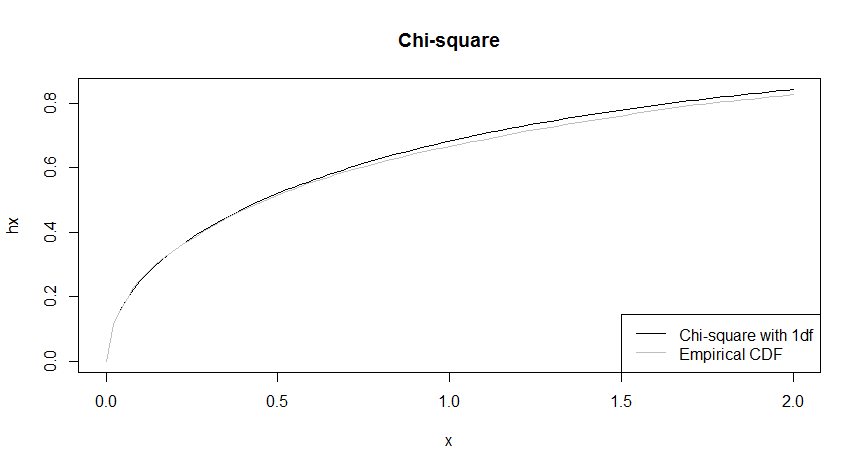
\includegraphics[width=15cm]{chi-square-emp.png}
				\end{center}

			\item Repeat the previous part, using a sample of size 100 instead of 25. Does the approximation improve?
				\begin{center}
					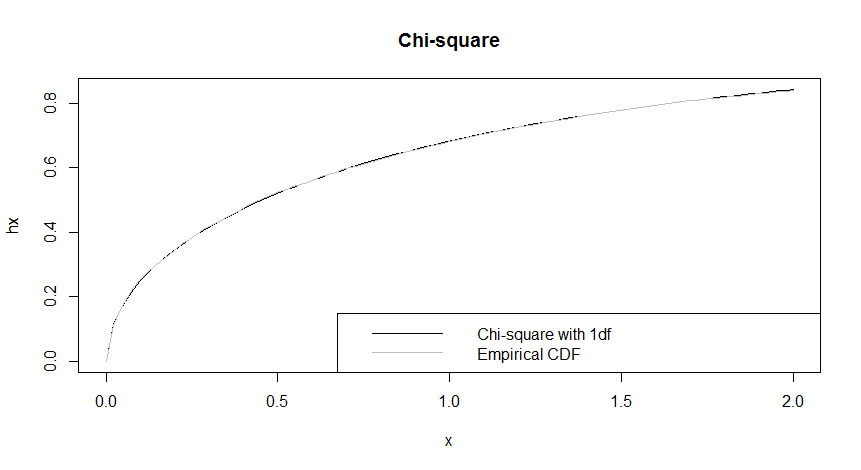
\includegraphics[width=15cm]{chi-square-emp-100.png}
				\end{center}	
				
		\end{enumerate}
\end{itemize}
\newpage

\section*{Chapter 11: Comparing Two Samples}

\begin{itemize}
	\item[1.] A computer was used to generated four random numbers from a normal distribution with a set mean and variance: 1.1650, 0.6268, 0.0751, 0.3516. Five more random normal numbers with the same variance but perhaps a different mean were then generated (the mean may or may not actually be different): 0.3035, 2.6961, 1.0591, 2.7971, 1.2641.
		\begin{enumerate}[a.]
			\item What do you think the means of the random normal number generators were? What do you think the difference of the means was?
				\begin{soln}
					Using the sample mean, the mean of the first RNG would be 0.5546. The mean of the second RNG would be 1.6240. The difference in means would be 1.0694.
				\end{soln}

			\item What do you think the variance of the random number generator was?
				\begin{soln}
					The variance of the first batch of numbers was 0.4651, and the sample variance of the second batch was 1.086. The pooled sample variance is given by \[\frac{3(0.4651) + 4(1.086)}{7} = 0.8199\] which would be the variance of the RNG.
				\end{soln}

			\item What is the estimated standard error of your estimate of the difference of the means?
				\begin{soln}
					The estimated standard error of the difference of means is given by \[s_p\sqrt{\frac{1}{n}+\frac{1}{m}} = \sqrt0.8199\cdot\sqrt{\frac{1}{4} + \frac{1}{5}} = 0.6074\]
				\end{soln}

			\item Form a 90\% confidence interval for the difference of the means of the random number generators.
				\begin{soln}
					The difference of means from part a was 1.0694, and we have $t_7(10/2)=1.895,$ so the 90\% confidence interval is given by \[1.0694\pm 1.895(0.6074)= (-0.0816, 2.2204)\]
				\end{soln}

			\item In this situation, is it more appropriate to use a one-sided test or a two-sided test of the equality of the means?
				\begin{answer*}
					It is more appropriate to use a two-sided test because we don't know anything about the means, and we already have a confidence interval.
				\end{answer*}

			\item What is the $p$-value of a two-sided test of the null hypothesis of equal means?
				\begin{soln}
					Under the null hypothesis, the means are equal, so the test statistic is \[t=\frac{\bar{X}-\bar{Y}}{s_p\sqrt{\frac{1}{n}+\frac{1}{m}}}=\frac{1.0694}{0.6074} = 1.7606\] Then since we have a $t$-distribution, the $p$-value is \[P(t<-1.7606) + P(t>1.7606) = 2(0.0608) = 0.1216\]
				\end{soln}

			\item Would the hypothesis that the means were the same versus a two-sided alternative be rejected at the significance level $\alpha=0.1?$
				\begin{answer*}
					No, since the $p$-value is not less than $\alpha,$ we do not reject the null hypothesis.
				\end{answer*}

			\item Suppose you know that the variance of the normal distribution was $\sigma^2=1.$ How would your answers to the preceding questions change?
				\begin{answer*}
					Instead of using the pooled sample variance, we could directly use the standard deviation. Then the test statistic would be a standard normal variable instead of a $t.$
				\end{answer*}
				
		\end{enumerate}

	\item[2.] The difference of the means of two normal distributions with equal variance is to be stimated by sampling an equal number of observations from each distribution. If it were possible, would it be better to halve the standard deviation of the populations or double the sample sizes?
		\begin{answer*}
			Let $X_i$ have distribution $N(\mu_X, \sigma_X^2)$ and $Y_i$ have distribution $N(\mu_Y, \sigma_Y^2).$ If we draw $n$ from each sample, then $\bar{X}-\bar{Y}$ has distribution $N\left( \mu_X-\mu_Y, \frac{\sigma_X^2+\sigma_Y^2}{n} \right).$ If we halve the SD of each sample, then this has the effect of reducing the variance of $\bar{X}-\bar{Y}$ by a factor of 4, while if we double the sample sizes, this only reduces the variance by a factor of 2. Thus, it would be better to halve the SD of the populations.
		\end{answer*}

	\item[3.] In Section 11.2.1, we considered two methods of estimating $\var(\bar{X}-\bar{Y}).$ Under the assumption that the two population variances were equal, we estimated this quantity by \[s_p^2\left( \frac{1}{n}+\frac{1}{m} \right)\] and without this assumption by \[\frac{s_X^2}{n}+\frac{s_Y^2}{m}\] Show that these two estimates are identical if $m=n.$
		\begin{proof}
			If $n=m,$ then we have
			\begin{align*}
				s_p^2\left( \frac{1}{n}+\frac{1}{m} \right) &= \frac{(n-1)s_X^2+(m-1)s_Y^2}{n+m-2} \left( \frac{1}{n}+\frac{1}{m} \right) \\
				&= \frac{(n-1)s_X^2 + (n-1)s_Y^2}{2(n-1)}\cdot\frac{2}{n} \\
				&= \frac{s_X^2+s_Y^2}{n} = \frac{s_X^2}{n} + \frac{s_Y^2}{n} \\
				&= \frac{s_X^2}{n} + \frac{s_Y^2}{m}
			\end{align*}
			as desired.
		\end{proof}

	\item[10.] Verify that the two-sample $t$ test at level $\alpha$ of $H_0:\mu_X=\mu_Y$ versus $H_A:\mu_X\neq\mu_Y$ rejects if and only if the confidence interval for $\mu_X-\mu_Y$ does not contain zero.
		\begin{proof}
			Suppose we are at the significance level $\alpha$ with $n+m-2$ degrees of freedom. The confidence interval for $\mu_X-\mu_Y$ is given by \[(\bar{X}-\bar{Y}) \pm t_{n+m-2}(\alpha/2) s_{\bar{X}-\bar{Y}}\] If the confidence interval does not contain 0, WLOG $\bar{X}>\bar{Y},$ then we have \[\frac{\bar{X}-\bar{Y}}{s_{\bar{X}-\bar{Y}}} > t_{n+m-2}(\alpha/2)\] However, this is exactly the condition where we reject the null hypothesis. Since each step here was invertible, the reverse direction holds as well.
		\end{proof}

	\item[11.] Explain how to modify the $t$ test of Section 11.2.1 to test $H_0: \mu_X=\mu_Y+\Delta$ versus $H_A: \mu_X\neq \mu_Y+\Delta$ where $\Delta$ is specified.
		\begin{answer*}
			In this case, we have \[t=\frac{(\bar{X}-\bar{Y})-(\mu_X-\mu_Y)}{s_{\bar{X}-\bar{Y}}}=\frac{\bar{X}-\bar{Y}-\Delta}{s_{\bar{X}-\bar{Y}}}\] under the null hypothesis. Everything else is the same.
		\end{answer*}
		
\end{itemize}

\section*{Chapter 12: The Analysis of Variance}

\begin{itemize}
	\item[2.] Verify that if $I=2,$ the estimate $s_p^2$ of Theorem $A$ of Section 11.2.1 is the $s_p^2$ given in Section 12.2.1.
		\begin{proof}
			The estimate $s_p^2$ of Theorem A Section 11.2.1 is given by \[s_p^2=\frac{(n-1)s_X^2+(m-1)s_Y^2}{n+m-2}\] and in section 12.2.1 it is \[s_p^2=\frac{SS_W}{I(J-1)} = \frac{1}{2(J-1)}\sum_{i=1}^{2}(J-1)s_i^2=\frac{s_1^2+s_2^2}{2}\] if $I=2.$ Then since $n=m$ in this assumption, the first estimate becomes \[s_p^2=\frac{s_X^2+s_Y^2}{2}\] and these two expressions are identical, as desired.
		\end{proof}

	\item[3.] For a one-way analysis of variance with $I=2$ treatment groups, show that the $F$ statistic is $t^2,$ where $t$ is the usual $t$ statistic for a two-sample case.
		\begin{proof}
			We have \[F=\frac{SS_B/(I-1)}{SS_W/(I(J-1)}\] and if $I=2,$ then the numerator is a chi-square variable with 1 degree of freedom, which is exactly $Z^2.$ A $t$ statistic is a ratio between a $Z$ and the square-root of a normalized chi-square variable, so squaring a $t$ yields this $F$ statistic, as desired.
		\end{proof}

	\item[4.] Prove the analogues of Theorems A and B in Section 12.2.1 for the case of unequal numbers of observations in the cells of a one-way layout.
		\begin{proof}[Theorem A]
			Suppose the $i$-th treatment has $f(i)$ observations. Then we have
			\begin{align*}
				E[SS_W] &= \sum_{i=1}^{I} \sum_{j=1}^{f(i)}E[(Y_{ij}-\bar{Y}_{i\cdot})^2] \\
				&= \sum_{i=1}^{I} \sum_{j=1}^{f(i)}\frac{f(i)-1}{f(i)}\sigma^2 = \sum_{i=1}^{I}(f(i)-1)\sigma^2
			\end{align*}
			Similarly, we have
			\begin{align*}
				E[SS_B] &= \sum_{i=1}^{I} \sum_{j=1}^{f(i)} E[(\bar{Y}_{i\cdot} - \bar{Y}_{\cdot\cdot})^2] \\
				&= \sum_{i=1}^{I} \sum_{j=1}^{f(i)} \left[ \alpha_i^2 + \frac{I-1}{If(i)}\sigma^2 \right] = \sum_{i=1}^{I} \left(f(i)\alpha_i^2 + \frac{I-1}{I}\sigma^2\right) \\
				&= (I-1)\sigma^2 + \sum_{i=1}^{I}f(i)\alpha_i^2
			\end{align*}
		\end{proof}

		\begin{proof}[Theorem B]
			We have \[\frac{1}{\sigma^2}\sum_{j=1}^{f(i)}(Y_{ij}-\bar{Y}_{i\cdot})^2\] follows a chi-square distribution with $f(i)-1$ degrees of freedom. We sum from $i=1$ to $i=I$ and these comprise $SS_W,$ and each is independent. The total number of degrees of freedom of these independent chi-square variables is \[\sum_{i=1}^{I} (f(i)-1)=-I+\sum_{i=1}^{I}f(i)\] Then the proof of the second part is identical to the proof in the book.
		\end{proof}
		
\end{itemize}

\end{document}
